\documentclass[12pt, oneside, a4paper]{ppgcc}

%******************* Importing packages *********************************************
\usepackage[utf8]{inputenc}
\usepackage[T1]{fontenc}
%\usepackage[brazilian,english]{babel}
\usepackage[brazil]{babel}
\usepackage{graphicx,url}
\usepackage{listings}
\usepackage{subfigure}
\usepackage{multirow}
\usepackage{amsmath,amsfonts,amscd,bezier,amssymb}
\usepackage{xspace}
\usepackage{setspace}
\usepackage{float}
\usepackage{placeins} % supporting figures placement
\usepackage{booktabs} % style for plain tables
\usepackage{colortbl} % for colouring tables
\usepackage{luximono}
\usepackage{slashbox}
\usepackage{microtype}
\usepackage{calligra}
\usepackage{lscape}
\usepackage{scalefnt}
\usepackage{lipsum}
\usepackage{pgfgantt} % para inserir o cronograma baseado no gráfico de Gantt
\usepackage[top=20mm,bottom=10mm,left=30mm,right=20mm,pdftex,includeheadfoot]{geometry}
\usepackage{times}
\usepackage{color}
\usepackage{colortbl}
\usepackage{verbatim}
\usepackage{textfit}
\usepackage{alltt}
\usepackage{ae}
\usepackage{fancyhdr}
\usepackage{fancybox}
\usepackage{multicol}
\usepackage{helvet}
\usepackage{paralist}
\usepackage{enumerate}
\usepackage{wasysym} % package for special symbols and emoticons
\usepackage{graphicx}
\usepackage{booktabs}
\usepackage{mathtools}
\usepackage{pdflscape}
\usepackage{lscape}
%\usepackage[table,xcdraw]{xcolor}
\usepackage{tabularx}
%\usepackage[scaled=0.9]{luximono} % import font
\usepackage[%numbers,
            authoryear,
            sort&compress,]{natbib}
\usepackage[pdftex]{hyperref}  % create hyperlinks in the pdf
\usepackage{pdfpages}
%\usepackage[usenames,dvipsnames,svgnames,table]{xcolor}


%*********************  Definindo novas cores  *******************************
\definecolor{verde}{rgb}{0.25,0.5,0.35}
\definecolor{jpurple}{rgb}{0.5,0,0.35}
\definecolor{Blue}{rgb}{0,0,0.9}
\definecolor{darkgreen}{cmyk}{1,0,1,0}


%*********************  Parâmetros  ******************************************

\titulo{Exemplo de título grande para ocupar mais de uma linha}
\autor{Fulano de Tal}
\orientador[Orientadora]{Profa. Dra. Fulana de Tal}
\coorientador[Co-orientadora]{Profa. Dra. Coorirentadora Fulana de Tal}
\dataDocumento{Maio/2018}
\tipodoc{Qualificação} %Dissertação/Qualificação/Tese 
\tipotitulo{Doutor} %Mestre/Doutor
\areaconcentracao{Engenharia de software}


%*********************  Parâmetros PDF ***************************************
\hypersetup{colorlinks=true,debug=false,
   linkcolor=black,%%% tableofcontents,\ref,\footnote,etc colour
   citecolor=black, %%% \cite colour
   urlcolor=black, %%% \url and \href colour
   pdftitle={\PPGtitulo},
   pdfauthor={\PPGautor},
   pdfsubject={\comentario}}

\pdfcompresslevel=9
\DeclareGraphicsExtensions{.png,.jpg,.pdf,.mps}




%*********************  Comandos ***************************************

% Configurando layout para mostrar codigos Java
%\lstset{language=[AspectJ]Java, basicstyle=\ttfamily\footnotesize,showstringspaces=false}
%\lstset{language=[AspectJ]Java,
%\lstset{language=Java,
%	basicstyle=\scriptsize,
%	keywordstyle=\color{black}\bfseries\scriptsize,
%	identifierstyle=\rmfamily\scriptsize, 
%	stringstyle=\ttfamily\scriptsize,
%	showstringspaces=false,
%	numbers=left, 
%	numberstyle=\tiny}
	
\lstset{
  language=Java,
  basicstyle= \ttfamily\scriptsize,  % tiny, scriptsize, footnotesize, small, normalsize, large, Large, huge, Huge
  keywordstyle=\color{jpurple}\bfseries,
  stringstyle=\color{red},
  commentstyle=\color{darkgreen},
  morecomment=[s][\color{blue}]{/**}{*/},
  extendedchars=true, 
  showspaces=false, 
  showstringspaces=false, 
  numbers=left,
  numberstyle=\tiny,
  breaklines=true, 
  backgroundcolor=\color{cyan!10}, 
  breakautoindent=true, 
  captionpos=b,
  xleftmargin=0pt,
  tabsize=4
}

%*****************************  new commands   ************************
% new colours
\definecolor{gray}{rgb}{0.85,0.85,0.85} % definição de cor cinza
\newcommand{\SetRowColor}[1]{\noalign{\gdef\RowColorName{#1}}\rowcolor{\RowColorName}}
\newcommand{\mymulticolumn}[3]{\multicolumn{#1}{>{\columncolor{\RowColorName}}#2}{#3}}
\definecolor{MyGray}{rgb}{0.85,0.85,0.85}
\definecolor{MyDarkGray}{rgb}{0.7,0.7,0.7}

%% languages
%
%\newcommand{\aspectj}{\normalfont{AspectJ}\xspace}
%\newcommand{\caesarj}{\normalfont{CaesarJ}\xspace}
%\newcommand{\aspectwerkz}{\normalfont{AspectWerkz}\xspace}
%\newcommand{\jbossaop}{\normalfont{JBossAOP}\xspace}
%\newcommand{\springaop}{\normalfont{SpringAOP}\xspace}
%\newcommand{\java}{\normalfont{Java}\xspace}
%\newcommand{\fortran}{\normalfont{Fortran}\xspace}
%\newcommand{\simula}{\normalfont{SIMULA}\xspace}
%\newcommand{\smalltalk}{\normalfont{Smalltalk}\xspace}
%\newcommand{\squeak}{\normalfont{Squeak}\xspace}
%\newcommand{\cansi}{\normalfont{C}\xspace}
%%\newcommand{\cplusplus}{\normalfont{C++}\xspace}
%\newcommand{\cplusplus}{\normalfont{C\footnotesize{++}}\xspace}
%\newcommand{\csharp}{\normalfont{C\#}\xspace}
%\newcommand{\pascal}{\normalfont{Pascal}\xspace}
%\newcommand{\objectpascal}{\normalfont{Object Pascal}\xspace}
%\newcommand{\modulatwo}{\normalfont{Modula-2}\xspace}
%\newcommand{\modulathree}{\normalfont{Modula-3}\xspace}
%\newcommand{\eiffel}{\normalfont{Eiffel}\xspace}
%\newcommand{\php}{\normalfont{PHP}\xspace}
%
%\newcommand{\aspectcplusplus}{\normalfont{AspectC\footnotesize{++}}\xspace}
%\newcommand{\aspectcansi}{\normalfont{AspectC}\xspace}
%\newcommand{\aspectcsharp}{\normalfont{AspectC\#}\xspace}
%\newcommand{\aspectsmalltalk}{\normalfont{AspectS}\xspace}
%\newcommand{\aophp}{\normalfont{AOPHP}\xspace}
%
%\newcommand{\y}{\rule{8pt}{7pt}}
%\newcommand{\x}{\hspace*{2pt}}
%
%% tools
%
%\newcommand{\proteum}{\emph{Proteum}\xspace}
%\newcommand{\proteumim}{\emph{Proteum/IM}\xspace}
%\newcommand{\proteumaj}{\emph{Proteum/AJ}\xspace}
%
%\newcommand{\start}{\emph{Start}\xspace}
%
%\newcommand{\jabuti}{\emph{JaBUTi}\xspace}
%\newcommand{\jabutiaj}{\emph{JaBUTi/AJ}\xspace}
%\newcommand{\jabutiweb}{\emph{JaBUTi/Web}\xspace}
%
%\newcommand{\mujava}{$\mu Java$\xspace}
%\newcommand{\mudel}{\emph{MuDel}\xspace}
%\newcommand{\mudelgen}{\emph{mudelgen}\xspace}
%\newcommand{\ajmutator}{\emph{AjMutator}\xspace}
%\newcommand{\ajte}{\emph{AJTE}\xspace}
%\newcommand{\aspectra}{\emph{Aspectra}\xspace}
%\newcommand{\jtest}{\emph{JTest}\xspace}
%\newcommand{\rostra}{\emph{Rostra}\xspace}
%\newcommand{\mutapro}{\emph{Muta-Pro}\xspace}
%\newcommand{\ajato}{\emph{AJATO}\xspace}
%
%
%\newcommand{\ant}{\emph{Ant}\xspace}
%\newcommand{\junit}{\emph{JUnit}\xspace}
%
%%\newcommand{\ibatis}{\emph{iBATIS}\xspace}
%%\newcommand{\hw}{\emph{HeathWatcher}\xspace}
%%\newcommand{\mm}{\emph{MobileMedia}\xspace}
%%\newcommand{\tsd}{\emph{Toll System Demonstrator}\xspace}
%
%\newcommand{\ibatis}{\element{iBATIS}\xspace}
%\newcommand{\hw}{\element{HealthWatcher}\xspace}
%\newcommand{\mm}{\element{MobileMedia}\xspace}
%\newcommand{\ajhd}{\element{AJHotDraw}\xspace}
%\newcommand{\ts}{\element{TollSystemDemonstrator}\xspace}
%
%
%\newcommand{\stratego}{\emph{Stratego/XT}\xspace}
%\newcommand{\aspectjfront}{\emph{AspectJ-front}\xspace}
%
%\newcommand{\aterm}{\textsf{aterm}\xspace}
%\newcommand{\ajc}{\textsf{ajc}\xspace}
%\newcommand{\abc}{\textsf{abc}\xspace}
%
%\newcommand{\rational}{\emph{IBM-Rational}\xspace}
%\newcommand{\poseidon}{\emph{Poseidon}\xspace}
%\newcommand{\argouml}{\emph{Argo-UML}\xspace}
%
%
%
%% others
%
%\newcommand{\refasset}{\emph{RefASSET}\xspace}
%\newcommand{\reftest}{\emph{RefTEST}\xspace}
%
%\newcommand{\framework}{\emph{framework}\xspace}
%\newcommand{\web}{\emph{Web}\xspace}
%\newcommand{\bytecode}{\normalfont{bytecode}\xspace}
%\newcommand{\bytecodes}{\normalfont{bytecodes}\xspace}
%\newcommand{\jvm}{\normalfont{JVM}\xspace}
%
%\newcommand{\cfg}{\textsf{CFG}\xspace}
%\newcommand{\icfg}{\textsf{ICFG}\xspace}
%\newcommand{\fcfg}{\textsf{FCFG}\xspace}
%\newcommand{\ccfg}{\textsf{CCFG}\xspace}
%\newcommand{\aocfg}{\textsf{AOCFG}\xspace}
%\newcommand{\aodu}{\textsf{AODU}\xspace}
%\newcommand{\pwdu}{\textsf{PWDU}\xspace}
%\newcommand{\pcdu}{\textsf{PCDU}\xspace}
%\newcommand{\madu}{\textsf{MADU}\xspace}
%\newcommand{\ig}{\textsf{IG}\xspace}
%\newcommand{\dug}{\textsf{DUG}\xspace}
%\newcommand{\defusegraph}{\emph{Def-Use Graph}\xspace}
%\newcommand{\fsm}{\textsf{FSM}\xspace}
%\newcommand{\free}{\textsf{FREE}\xspace}
%\newcommand{\asm}{\textsf{ASM}\xspace}



%%%% COLOURED - inserted by Fabiano
%\newcommand{\bento}[1]{{{\color{black} #1}}}
%\newcommand{\alessandro}[1]{{\color{black} #1}}
%\newcommand{\alessandroNew}[1]{{\color{black} #1}}
%\newcommand{\fabiano}[1]{{\color{black} #1}}
%\newcommand{\important}[1]{{\color{red} [IMPORTANTE: #1]}}
%\newcommand{\fabianonew}[1]{{\color{black} #1}}
%
%\newcommand{\rever}[1]{{\color{red} #1}}
%\newcommand{\novo}[1]{{\color{blue} #1}}



% with parameters
% Setting tables
	\newcommand{\confTab}{
	\fontencoding{T1}
 	\fontfamily{\sfdefault}
	\fontseries{m}
	\fontshape{n}
	\fontsize{10}{15}
	\selectfont
	\rowcolors{2}{}{lightgray!30}
	\centering
}

\renewcommand{\lstlistingname}{Listagem de Código}% Listing -> Algorithm
\renewcommand{\lstlistlistingname}{Listagens de Códigos}% List of Listings -> List of Algorithms


\newcommand{\blue}[1]{{{\color{blue} #1}}}
\newcommand{\red}[1]{{{\color{red} #1}}}
\newcommand{\code}[1]{{\texttt{#1}}}
\newcommand{\wild}[1]{{``\texttt{#1}''}}
\newcommand{\opname}[1]{{\textsf{#1}}}
\newcommand{\smallop}[1]{{\small\textsf{#1}}}
%\newcommand{\fault}[1]{{\footnotesize\textsf{#1}}}
\newcommand{\fault}[1]{{\textsf{#1}}}
\newcommand{\element}[1]{{\textsf{#1}}}
\newcommand{\concept}[1]{{\textbf{\emph{#1}}}}
\newcommand{\declare}{\code{declare}}


%*****************************  style definitions   ************************

\widowpenalty=10000
\clubpenalty=10000
\exhyphenpenalty=10000

% defining space between figures, captions and text
\setlength{\abovecaptionskip}{0.2cm}
\setlength\textfloatsep{12pt}
\setlength\floatsep{12pt}

\headheight 17.1pt

\setcounter{secnumdepth} {3} % Adjusting number of levels
\setcounter{tocdepth} {3} % Adjusting number of levels in table of contents


%*********************  Documento  ******************************************
% Estrutura: https://www.mindomo.com/pt/mindmap/mapadissertacaosandra-1cf625c9dea942e4b315aa3a2d9e10b5

\begin{document}

%*********************  Elementos pré-textuais  *****************************
% Agradecimentos, Resumo, Abstract, Índices, Abreviaturas

\pagestyle{empty}
\thispagestyle{empty}
\let\cite=\citep    			% defines citation style
\cleardoublepage

%%% CAPA
\capa


%%% FOLHA DE ROSTO
\rosto


%%% VERSO DA FOLHA DE ROSTO
%Não é necessária por enquanto


%%% FOLHA DE APROVAÇÃO
%Não é necessária por enquanto


%%% DEDICATÓRIA
\dedicatoria{Dedico à Fulano.}


% Inicia a numeração das páginas
\newpage
\pagestyle{plain}
\thispagestyle{plain}
\renewcommand{\thepage}{\roman{page}}
\setcounter{page}{1}


%%% AGRADECIMENTOS
\agradecimentos{
	\lipsum[1-2]
}

%%% EPÍGRAFE
\epigrafe{
Lorem ipsum dolor sit amet, consectetur adipiscing elit, sed do eiusmod tempor incididunt ut labore et dolore magna aliqua. Ut enim ad minim veniam, quis nostrud exercitation ullamco laboris nisi ut aliquip ex ea commodo consequat. Duis aute irure dolor in reprehenderit in voluptate velit esse cillum dolore eu fugiat nulla pariatur.
}
{Autor da Epígrafe}


%%% RESUMO PORTUGUES
\resumo{
    \textbf{\textit{Contexto}}: Lorem ipsum dolor sit amet, consectetur adipiscing elit, sed do eiusmod tempor incididunt ut labore et dolore magna aliqua. Ut enim ad minim veniam, quis nostrud exercitation ullamco laboris nisi ut aliquip ex ea commodo consequat. Duis aute irure dolor in reprehenderit in voluptate velit esse cillum dolore eu fugiat nulla pariatur. 
    \textbf{\textit{Objetivos}}: Lorem ipsum dolor sit amet, consectetur adipiscing elit, sed do eiusmod tempor incididunt ut labore et dolore magna aliqua. Ut enim ad minim veniam, quis nostrud exercitation ullamco laboris nisi ut aliquip ex ea commodo consequat. Duis aute irure dolor in reprehenderit in voluptate velit esse cillum dolore eu fugiat nulla pariatur. 
    \textbf{\textit{Metodo}}:Lorem ipsum dolor sit amet, consectetur adipiscing elit, sed do eiusmod tempor incididunt ut labore et dolore magna aliqua. Ut enim ad minim veniam, quis nostrud exercitation ullamco laboris nisi ut aliquip ex ea commodo consequat. Duis aute irure dolor in reprehenderit in voluptate velit esse cillum dolore eu fugiat nulla pariatur. 
    \textbf{\textit{Resultados}}: Lorem ipsum dolor sit amet, consectetur adipiscing elit, sed do eiusmod tempor incididunt ut labore et dolore magna aliqua. Ut enim ad minim veniam, quis nostrud exercitation ullamco laboris nisi ut aliquip ex ea commodo consequat. Duis aute irure dolor in reprehenderit in voluptate velit esse cillum dolore eu fugiat nulla pariatur. 
    \textbf{\textit{Conclusão}}: Lorem ipsum dolor sit amet, consectetur adipiscing elit, sed do eiusmod tempor incididunt ut labore et dolore magna aliqua. Ut enim ad minim veniam, quis nostrud exercitation ullamco laboris nisi ut aliquip ex ea commodo consequat. Duis aute irure dolor in reprehenderit in voluptate velit esse cillum dolore eu fugiat nulla pariatur. 
}
{chave 1, chave 2, chave 3, chave 4, chave 5, chave 6, chave 7, chave 8, chave 9, chave 10, chave 11, chave 12, chave 13, chave 14, chave 15, chave 16, chave 17, chave 18, chave 19, chave 20}


%%% RESUMO INGLES
\abstract{
    \textbf{\textit{Context}}: Lorem ipsum dolor sit amet, consectetur adipiscing elit, sed do eiusmod tempor incididunt ut labore et dolore magna aliqua. Ut enim ad minim veniam, quis nostrud exercitation ullamco laboris nisi ut aliquip ex ea commodo consequat. Duis aute irure dolor in reprehenderit in voluptate velit esse cillum dolore eu fugiat nulla pariatur. 
    \textbf{\textit{Objective}}: Lorem ipsum dolor sit amet, consectetur adipiscing elit, sed do eiusmod tempor incididunt ut labore et dolore magna aliqua. Ut enim ad minim veniam, quis nostrud exercitation ullamco laboris nisi ut aliquip ex ea commodo consequat. Duis aute irure dolor in reprehenderit in voluptate velit esse cillum dolore eu fugiat nulla pariatur. 
    \textbf{\textit{Method}}:Lorem ipsum dolor sit amet, consectetur adipiscing elit, sed do eiusmod tempor incididunt ut labore et dolore magna aliqua. Ut enim ad minim veniam, quis nostrud exercitation ullamco laboris nisi ut aliquip ex ea commodo consequat. Duis aute irure dolor in reprehenderit in voluptate velit esse cillum dolore eu fugiat nulla pariatur. 
    \textbf{\textit{Results}}: Lorem ipsum dolor sit amet, consectetur adipiscing elit, sed do eiusmod tempor incididunt ut labore et dolore magna aliqua. Ut enim ad minim veniam, quis nostrud exercitation ullamco laboris nisi ut aliquip ex ea commodo consequat. Duis aute irure dolor in reprehenderit in voluptate velit esse cillum dolore eu fugiat nulla pariatur. 
    \textbf{\textit{Conclusão}}: Lorem ipsum dolor sit amet, consectetur adipiscing elit, sed do eiusmod tempor incididunt ut labore et dolore magna aliqua. Ut enim ad minim veniam, quis nostrud exercitation ullamco laboris nisi ut aliquip ex ea commodo consequat. Duis aute irure dolor in reprehenderit in voluptate velit esse cillum dolore eu fugiat nulla pariatur. 
}
{key1, key2, key3, key4, key5, key6, key7, key8, key9, key10, key11, key12, key13, key14, key15, key16, key17, key18, key19, key20}


%%% listas
%\lstlistoflistings


%%% FIGURAS
\listoffigures


%%% TABELAS
\listoftables


%%% ABREVIATURAS E SIGLAS
\begin{abbreviations}
	
	\begin{table}[!ht]
	\setlength{\tabcolsep}{3pt}
	\centering
		\begin{tabular}{  l p{13cm}  } 
			 \textbf{BPMN}   & \textit{Business Process Model Notation} \\
		\end{tabular}
	\end{table}

\end{abbreviations}


%%% SUMARIO
\renewcommand\contentsname{Sumário}
\tableofcontents

%***********************************************************************************
%**************************** FORMATAÇÃO DOS CAPÍTULOS *****************************
%***********************************************************************************

\clearpage{\pagestyle{empty}\cleardoublepage}

%\newpage
\onehalfspace
%\doublespace
%\linespread{1.35}

%% from quali.tex
%\pagestyle{fancy}   			% defines the page style
%\fancyfoot[C]{\thepage}  		% insert page number in the footer
%\fancyhead[R]{\small\leftmark}
%\lhead{}            			% defines right side of heading as empty
%\chead{}						% defines centre of heading as empty

\pagestyle{fancy}   								% defines the page style
\fancyhead{}										% cleaning-up previous settings

\fancyhead[L,R]{\textsl{\leftmark}}
\rhead{\sffamily\thepage\space}

%\fancyhead[LE]{\nouppercase{\slshape \rightmark}} 	% inserts the section name in the header of even pages
%\fancyhead[RO]{\nouppercase{\slshape \leftmark}}  	% inserts the chapter name in the header of odd pages
%\cfoot{\thepage}	
\cfoot{}											% clear the footer
\renewcommand{\headrulewidth}{1pt}					% defining header and footer rules
%\renewcommand{\footrulewidth}{1pt}


%*******************************************************************************

\newpage
\renewcommand{\thepage}{\arabic{page}}
\setcounter{page}{1}
\renewcommand{\chaptermark}[1]{\markboth{\textit{ \chaptername \ \thechapter.\ #1}}{}}



%********************************************************************************
%*************** CAPÍTULOS ******************************************************
%********************************************************************************

\chapter{Capítulo de exemplo}\label{cap:exemplo}
\normalsize
\begin{resumoCapitulo}
\textbf{(Resumo opcional no início dos capítulos)} Aqui deve-se escrever um resumo bem pequeno sobre do que se trata o capítulo. O Capítulo XXXX trata dos assuntos x, y, z. Está estruturado da seguinte maneira: Contexto, Motivação, Objetivos, Metodologia e Organização. Se os textos de Objetivos e Metodologia forem pequenos, essas duas seções podem ser agregadas em uma só.
\end{resumoCapitulo}

\section{Exemplo de seção normal} \label{sec:Cap1-Secao1}
\lipsum[1]

\section{Exemplo de seção com o nome muito grande para ocupar mais de uma linha} \label{sec:Cap1-Secao2}
\lipsum[1]

\section{Exemplo de subseções} \label{sec:Cap1-Secao3}

\subsection{Subseção 1.3.1} \label{sec:Cap1-Secao1.3.1}
\lipsum[1]

\subsubsection{SubSubSeção 1.3.1.1} \label{sec:Cap1-Secao1.3.1.1}
\lipsum[1]

\subsection{Subseção 1.3.2} \label{sec:Cap1-Secao1.3.2}
\lipsum[1]

\section{Enumerações} \label{sec:Cap1-Secao4}
\subsection{Itemize}
Certamente o comando mais usado por mim em apresentações, pois trás estrutura de tópicos que é marca caracteristicas de apresentações em slide. O ambiente é muito simples,

\begin{itemize}
	\item Item 1
	\item Item 2
\end{itemize}

\subsection{Enumerate}
Um ambiente muito semelhante ao itemize é o enumerate, a única diferença é a utilização de números ou letras para classificar os itens, ao invés de pontos. Exmplo abaixo mostra a situação:

\begin{enumerate}
   \item item1
   \item item2
 \end{enumerate}

ou:

\begin{enumerate}[a]
	\item Preenchimento com \'Oxido de grafeno
	\item Aquecimento e redu\c{c}\~ao
	\item Desprotegimento do grafeno
	\item Secagem
	\item Remo\c{c}\~ao do Cobre
\end{enumerate}

\subsection{Descrição}
Uma terceira forma de listar é descrevendo os tópicos (pense em um glossário). Fazemos isso com o ambiente description:
\begin{description}
	\item[banana] fruta amarela, a forma lembra a Lua.
	\item[maçã] fruta vermelha e arredondada.
\end{description}

\section{Notas de rodapé} \label{sec:Cap1-rodape}

Criar uma nota de rodapé é simples\footnote{Esse é um exemplo de nota de rodapé.}.

\section{Referências} \label{sec:Cap1-Secao5}
Esse documento usa a biblioteca natbib para a gerenciamento das citações. Para mais exemplos do uso da biblioteca, favor acessar: \url{http://merkel.texture.rocks/Latex/natbib.php}.
\subsection{Citações básicas}
Existem duas formas básicas de citação: citet (para citação textual) e citep (para citação com parêntese). Existe também as versões com * as quais imprimem a lista completa de autores. Todas essas formas podem possuir até 2 argumentos (opcional) para adicionar um texto antes e depois da citação. 
\begin{description}
   \item [\textbackslash citet\{Acree1979\}]= \citet{Acree1979}
   \item [\textbackslash citet{[}capítulo 2{]} \{Acree1979\}]= \citet[capítulo 2]{Acree1979}
   \item [\textbackslash citep\{Acree1979\}]= \citep{Acree1979}
   \item [\textbackslash citep{[}capítulo 2{]}\{Acree1979\}]= \citep[capítulo 2]{Acree1979}
   \item [\textbackslash citep{[}veja{]}{[} {]}\{Acree1979\}]= \citep[veja][]{Acree1979}
   \item [\textbackslash citep{[}veja{]}{[}capítulo 2{]}\{Acree1979\}]= \citep[veja][capítulo 2]{Acree1979}
   \item [\textbackslash citet*\{Acree1979\}]= \citet*{Acree1979}
   \item [\textbackslash citep*\{Acree1979\}]= \citep*{Acree1979}
\end{description}

\subsection{Múltipas citações}
Citando mais de um trabalho de uma vez:
\begin{description}
   \item [\textbackslash citet\{Acree1979,lucredio2009\}]= \citet{Acree1979,lucredio2009}
   \item [\textbackslash citep\{Acree1979,lucredio2009\}]= \citep{Acree1979,lucredio2009}
   \item [\textbackslash citep\{Acree1979,Acree1980\}]= \citep{Acree1979,Acree1980}
   \item [\textbackslash citep\{Acreed1979a,Acreed1979b\}]= \citep{Acreed1979a,Acreed1979b}
\end{description}

\subsection{Citações parciais}
As vezes é necessário citar só parte da referência:

\begin{description}
   \item [\textbackslash citeauthor\{Acree1979\}] = \citeauthor{Acree1979}
   \item [\textbackslash citeauthor*\{Acree1979\}] = \citeauthor*{Acree1979}
   \item [\textbackslash citeyear\{Acree1979\}] = \citeyear{Acree1979}
   \item [\textbackslash citeyearpar\{Acree1979\}]= \citeyearpar{Acree1979}
\end{description}

\section{Figuras} \label{sec:Cap1-Secao6}
Recomenda-se deixar as figuras salvas em uma pasta dentro de cada capítulo, como nesse exemplo.
\begin{figure}[!ht]
	\centering
	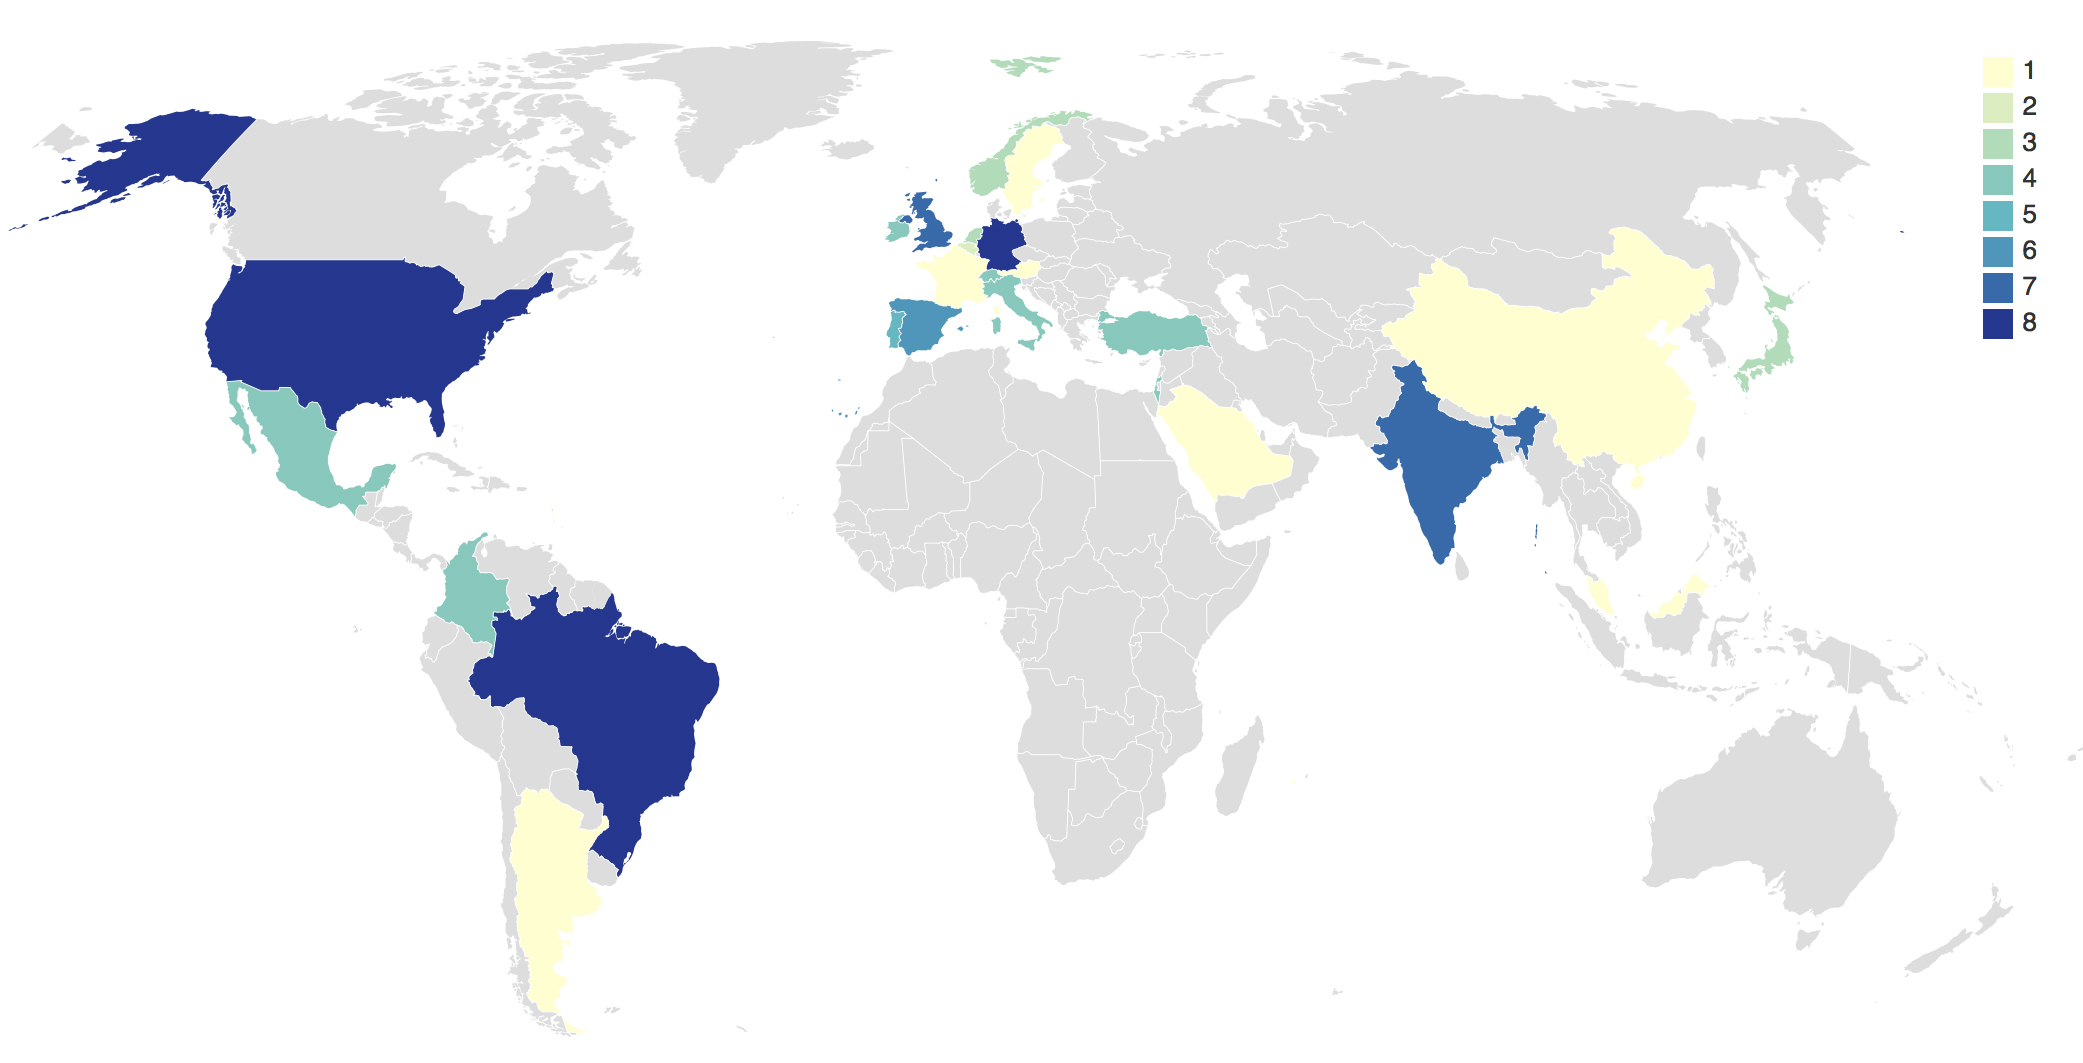
\includegraphics[width=1\textwidth]{Capitulo-1-Exemplo/Figuras/mapa.jpg}
	\caption{Exemplo de uso de Figura}
	\label{Start01}
\end{figure}

\lipsum[1]

\section{Tabelas} \label{sec:Cap1-Secao7}
Recomenda-se deixar as tabelas em arquivos separados e incluí-las como nesse exemplo.
\begin{table}[!ht]

%   float placement
%----------------------
%-h means here: Place the figure in the text where the figure environment is written, if there is enough room left on the page
%-t means top: Place it at the top of a page.
%-b means bottom: Place it at the bottom of a page.
%-p means page: Place it on a page containing only floats, such as figures and tables.
%-! allows to ignore certain parameters of LaTeX for float placement, for example:
%
%	\topfraction: maximal portion of a page (or column resp., here and below), which is allowed to be used by floats at its top, default 0.7
%	\bottomfraction: maximal portion of a page, which is allowed to be used by floats at its bottom, default value 0.3
%	\textfraction: minimal portion of a page, which would be used by body text, default value 0.2
%	\floatpagefraction: minimal portion of a float page, which has to be filled by floats, default value 0.2. This avoids too much white space on float pages.
%	topnumber: maximal number of floats allowed at the top of a page, default 2
%	bottomnumber: maximal number of floats allowed at the bottom of a page, default 1
%	totalnumber: maximal number of floats allowed at whole page, default 3

\setlength{\arrayrulewidth}{2\arrayrulewidth}  % line thickness
\setlength{\tabcolsep}{4pt} % spacing between columns
\centering

\caption{Exemplo de uso de tabelas}
\label{tablePaises}

%\fontencoding{T1}
%\fontfamily{\rmdefault}
\fontseries{m}
\fontshape{n}
%\fontsize{7.75}{8.5}
\selectfont
	\begin{tabular}{lclc}
		\toprule
		Country           & Number & Country         & Number \\ \midrule
		Germany        & 8          & USA          & 8          \\
		Brazil         & 7          & India        & 7          \\
		United Kingdom & 7          & Spain        & 6          \\
		Portugal       & 5          & Colombia     & 4          \\
		Ireland        & 4          & Israel       & 4          \\
		Italy          & 4          & Mexico       & 4          \\
		Switzerland    & 4          & Turkey       & 4          \\
		Japan          & 3          & Netherlands  & 3          \\
		Norway         & 3          & Belgium      & 2          \\
		Argentina      & 1          & Austria      & 1          \\
		China          & 1          & France       & 1          \\
		Malaysia       & 1          & Saudi Arabia & 1          \\
		Sweden         & 1          &              &            \\ \bottomrule
	\end{tabular}
\end{table}



\lipsum[1]



%********************************************************************************
%********************************************************************************

\chapter{Fundamentação teórica}\label{cap:fundamentos} 
\normalsize
\begin{resumoCapitulo}
\textbf{(Resumo opcional no início dos capítulos)} Aqui deve-se escrever um resumo bem pequeno sobre do que se trata o capítulo. O Capítulo XXXX trata dos assuntos x, y, z. Está estruturado da seguinte maneira: Contexto, Motivação, Objetivos, Metodologia e Organização. Se os textos de Objetivos e Metodologia forem pequenos, essas duas seções podem ser agregadas em uma só.
\end{resumoCapitulo}

\section{Seção1} \label{sec:Cap2-Secao1}
\lipsum[1]

\section{Seção2} \label{sec:Cap2-Secao2}
\lipsum[1]


%********************************************************************************
%********************************************************************************

\chapter{Revisão Sistemática}\label{cap:revisao} 
\normalsize
\begin{resumoCapitulo}
\textbf{(Resumo opcional no início dos capítulos)} Aqui deve-se escrever um resumo bem pequeno sobre do que se trata o capítulo. O Capítulo XXXX trata dos assuntos x, y, z. Está estruturado da seguinte maneira: Contexto, Motivação, Objetivos, Metodologia e Organização. Se os textos de Objetivos e Metodologia forem pequenos, essas duas seções podem ser agregadas em uma só.
\end{resumoCapitulo}

\section{Seção1} \label{sec:Cap3-Secao1}
\lipsum[1]

\section{Seção2} \label{sec:Cap3-Secao2}
\lipsum[1]


%********************************************************************************
%********************************************************************************

\chapter{Proposta de Pesquisa}\label{cap:proposta} 
\normalsize
\begin{resumoCapitulo}
\textbf{(Resumo opcional no início dos capítulos)} Aqui deve-se escrever um resumo bem pequeno sobre do que se trata o capítulo. O Capítulo XXXX trata dos assuntos x, y, z. Está estruturado da seguinte maneira: Contexto, Motivação, Objetivos, Metodologia e Organização. Se os textos de Objetivos e Metodologia forem pequenos, essas duas seções podem ser agregadas em uma só.
\end{resumoCapitulo}

\section{Seção1} \label{sec:Cap4-Secao1}
\lipsum[1]

\section{Seção2} \label{sec:Cap4-Secao2}
\lipsum[1]


%********************************************************************************
%******************  Bibliografia  **********************************************
%********************************************************************************

%\bibliographystyle{ppgcc2EN}
\bibliographystyle{ppgcc}
\newpage
\bibliografia
\renewcommand{\bibname}{\textbf{Refer\^encias}}
%\citeoption{abnt-etal-cite=2,abnt-etal-list=0}
\bibliography{references}


%********************************************************************************
%******************** APÊNDICES *************************************************
%********************************************************************************

\clearpage{}
\appendix
%\addcontentsline{toc}{chapter}{Apêndice}
\renewcommand{\chaptername}{Ap\^endice} % para colocar escrito Apêndice no cabeçalho

\chapter{Ferramenta StArt}\label{cap:ferramentaStart}
\thispagestyle{empty}
A ferramenta StArt -- \textit{State of the Art through Systematic Review} \cite{fabbri2013} -- foi desenvolvida para fornecer suporte computacional para o maior número possível de atividades de uma Revisão Sistemática, desde o preenchimento do protocolo na fase de planejamento, passando pelas atividades de seleção inicial e extração de dados na fase de execução, até a fase de sumarização dos dados.

\begin{enumerate}

    \item \textbf{Fase de Planejamento}
    
    Em relação ao planejamento, o protocolo trazido pela ferramenta possui os mesmos campos propostos por \citet{Kitchenham2011} para auxiliar os pesquisadores na condução da revisão sistemática e também na repetitividade do processo. Permite o registro de informações tais como objetivo, questões de pesquisa, métodos utilizados para seleção, palavras-chave utilizadas nas strings de busca, critérios de inclusão e exclusão, máquinas de busca utilizadas, formulário de extração, descrição de critérios de qualidade e de como a sumarização será feita. A \textit{Figura \ref{Start01}} mostra alguns campos do protocolo existente na ferramenta.
    
    \begin{figure}[!htb]
	\centering
	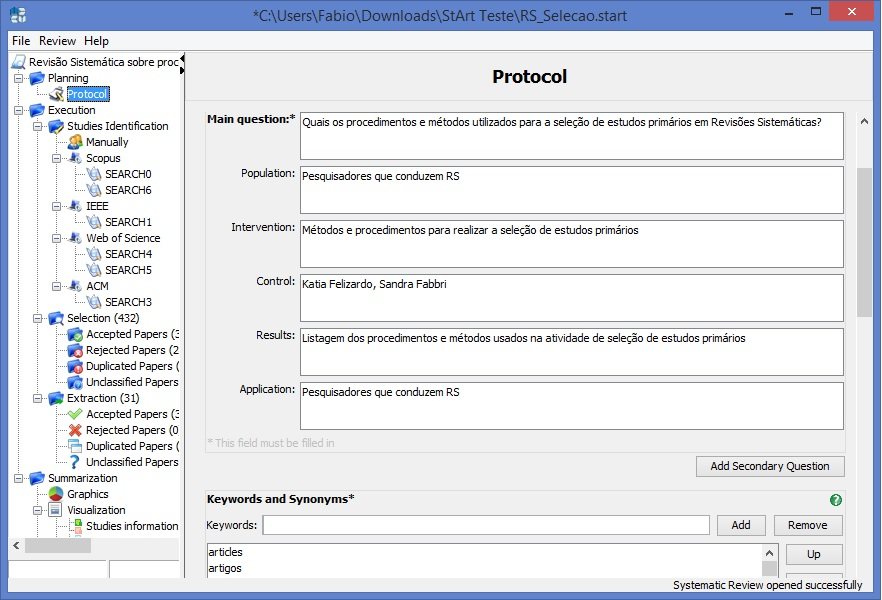
\includegraphics[scale=0.65]{Capitulo-Apendices/figura/Start01.jpg}
	\caption{Formulário de protocolo da ferramenta StArt}
	\label{Start01}
    \end{figure}
    
    \item \textbf{Fase de Execução}
    
    Em relação à execução, a ferramenta permite que os estudos primários recuperados das máquinas de busca sejam carregados por meio de arquivos exportados de várias máquinas de busca no formato BibTex, RIS, MedLine ou Cochrane. Artigos duplicados são detectados automaticamente pela ferramenta por meio de técnicas de mineração de texto.
    
    Além disso, a StArt traz um importante recurso para auxiliar os pesquisadores na seleção inicial de estudos primários: o score. Esse recurso considera a frequência com que as \textit{keywords} definidas no protocolo aparecem no título, \textit{abstract} e palavras-chave dos estudos primários recuperados, fazendo um ranqueamento de estudos. Quanto maior o score de um estudo, maior é a sua chance de ser relevante ao tema de pesquisa. A \textit{Figura \ref{Start02}} mostra um exemplo de tela da StArt no qual os estudos são classificados por score.
    
    \begin{figure}[!htb]
	\centering
	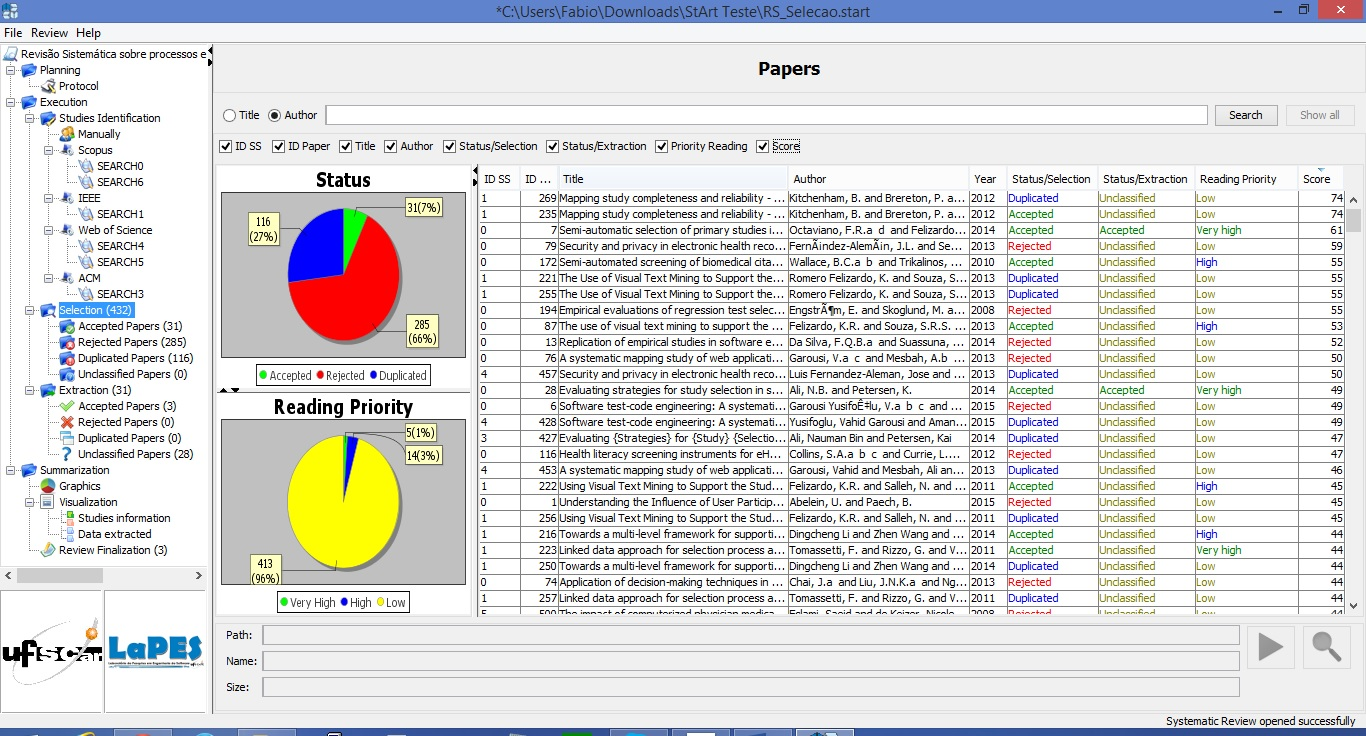
\includegraphics[scale=0.45]{Capitulo-Apendices/figura/Start02.jpg}
	\caption{Estudos classificados por score na atividade de seleção inicial}
	\label{Start02}
    \end{figure}
    
    Um recurso adicional que foi implementado e está em fase de aprimoramento é o número de citações entre os estudos primários (cross-citation) carregados na ferramenta. 
    
    Outro recurso existente que pode auxiliar o pesquisador na seleção é o percentual de similaridade de estudos, em que, por meio de mineração de texto, a ferramenta apresenta estudos similares em conteúdo em relação a um estudo selecionado pelo pesquisador. Assim, ao detectar um estudo relevante, é possível navegar por outros estudos com conteúdo similares, que supostamente tendem a ser relevantes também.

    Na etapa de extração, a ferramenta apresenta os campos do formulário de extração definido no protocolo para que as mesmas informações sejam extraídas de todos os estudos.
    
    \item \textbf{Fase de Sumarização dos Dados}
    
    Em relação à sumarização, a StArt apresenta funcionalidades para facilitar a sumarização dos dados, tais como o uso de recursos de visualização e a geração de relatórios no formato Excel de acordo com as necessidades do pesquisador. É possível gerar visualizações nos formatos de grafo, árvore e grafo-radial, e por diversos campos, tais como ano de publicação, autores, locais de eventos, campos do formulário de extração, entre outros.
    
\end{enumerate}


%********************************************************************************
%******************** ANEXOS ****************************************************
%********************************************************************************

\clearpage{}
\attachment
%\addcontentsline{toc}{chapter}{Anexo}
\renewcommand{\chaptername}{Anexo} % para colocar escrito Apêndice no cabeçalho

\chapter{Anexo da Ferramenta StArt} \label{cap:anexo1}
\thispagestyle{empty}
A ferramenta StArt -- \textit{State of the Art through Systematic Review} \cite{fabbri2013} -- foi desenvolvida para fornecer suporte computacional para o maior número possível de atividades de uma Revisão Sistemática, desde o preenchimento do protocolo na fase de planejamento, passando pelas atividades de seleção inicial e extração de dados na fase de execução, até a fase de sumarização dos dados.

\begin{enumerate}

    \item \textbf{Fase de Planejamento}
    
    Em relação ao planejamento, o protocolo trazido pela ferramenta possui os mesmos campos propostos por \citet{Kitchenham2011} para auxiliar os pesquisadores na condução da revisão sistemática e também na repetitividade do processo. Permite o registro de informações tais como objetivo, questões de pesquisa, métodos utilizados para seleção, palavras-chave utilizadas nas strings de busca, critérios de inclusão e exclusão, máquinas de busca utilizadas, formulário de extração, descrição de critérios de qualidade e de como a sumarização será feita. A \textit{Figura \ref{Start01}} mostra alguns campos do protocolo existente na ferramenta.
    
    \begin{figure}[!htb]
	\centering
	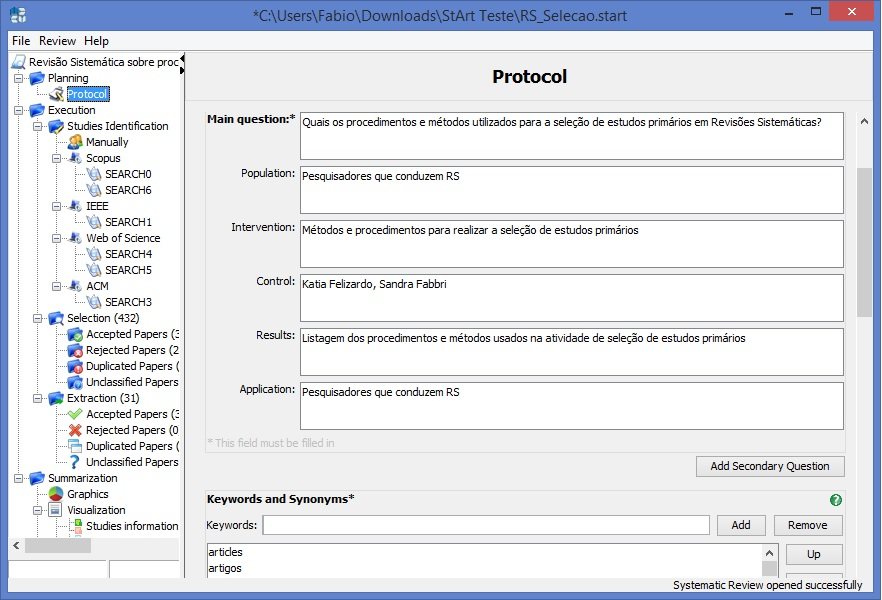
\includegraphics[scale=0.65]{Capitulo-Apendices/figura/Start01.jpg}
	\caption{Formulário de protocolo da ferramenta StArt}
	\label{Start01}
    \end{figure}
    
    \item \textbf{Fase de Execução}
    
    Em relação à execução, a ferramenta permite que os estudos primários recuperados das máquinas de busca sejam carregados por meio de arquivos exportados de várias máquinas de busca no formato BibTex, RIS, MedLine ou Cochrane. Artigos duplicados são detectados automaticamente pela ferramenta por meio de técnicas de mineração de texto.
    
    Além disso, a StArt traz um importante recurso para auxiliar os pesquisadores na seleção inicial de estudos primários: o score. Esse recurso considera a frequência com que as \textit{keywords} definidas no protocolo aparecem no título, \textit{abstract} e palavras-chave dos estudos primários recuperados, fazendo um ranqueamento de estudos. Quanto maior o score de um estudo, maior é a sua chance de ser relevante ao tema de pesquisa. A \textit{Figura \ref{Start02}} mostra um exemplo de tela da StArt no qual os estudos são classificados por score.
    
    \begin{figure}[!htb]
	\centering
	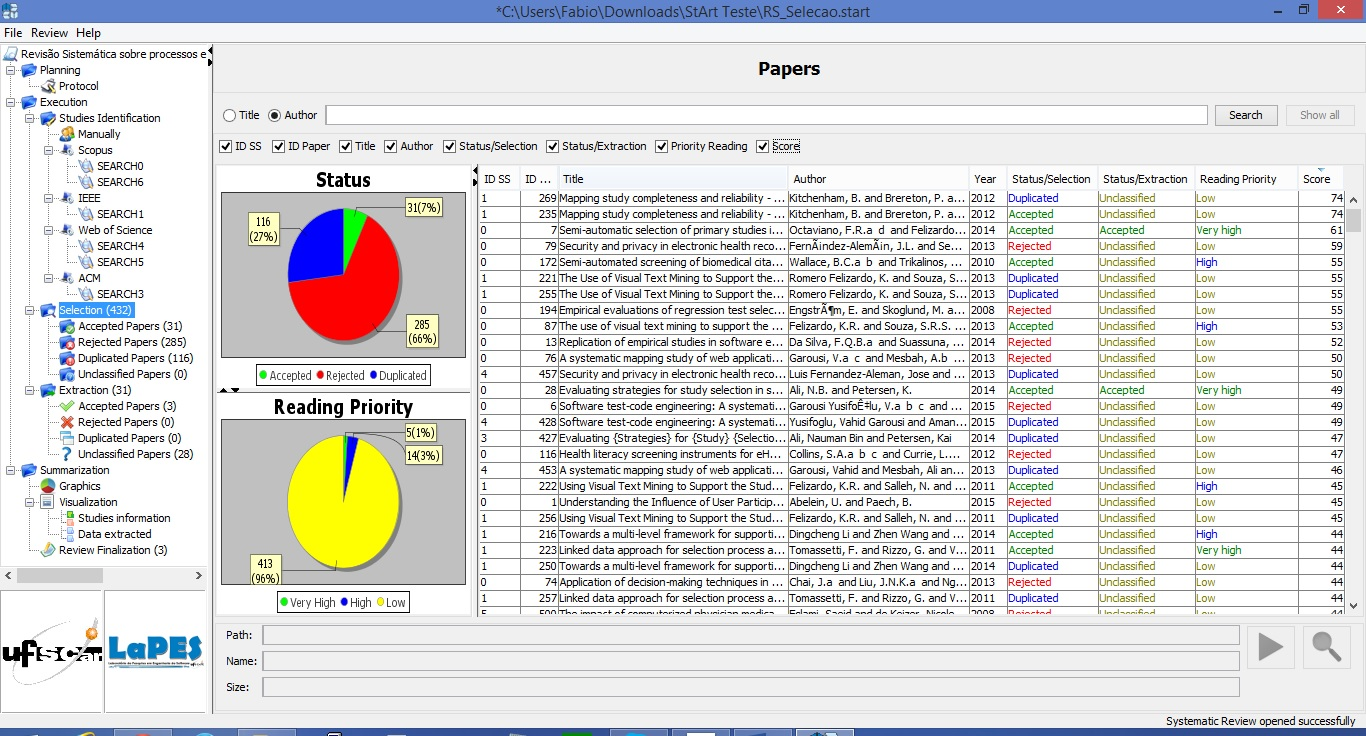
\includegraphics[scale=0.45]{Capitulo-Apendices/figura/Start02.jpg}
	\caption{Estudos classificados por score na atividade de seleção inicial}
	\label{Start02}
    \end{figure}
    
    Um recurso adicional que foi implementado e está em fase de aprimoramento é o número de citações entre os estudos primários (cross-citation) carregados na ferramenta. 
    
    Outro recurso existente que pode auxiliar o pesquisador na seleção é o percentual de similaridade de estudos, em que, por meio de mineração de texto, a ferramenta apresenta estudos similares em conteúdo em relação a um estudo selecionado pelo pesquisador. Assim, ao detectar um estudo relevante, é possível navegar por outros estudos com conteúdo similares, que supostamente tendem a ser relevantes também.

    Na etapa de extração, a ferramenta apresenta os campos do formulário de extração definido no protocolo para que as mesmas informações sejam extraídas de todos os estudos.
    
    \item \textbf{Fase de Sumarização dos Dados}
    
    Em relação à sumarização, a StArt apresenta funcionalidades para facilitar a sumarização dos dados, tais como o uso de recursos de visualização e a geração de relatórios no formato Excel de acordo com as necessidades do pesquisador. É possível gerar visualizações nos formatos de grafo, árvore e grafo-radial, e por diversos campos, tais como ano de publicação, autores, locais de eventos, campos do formulário de extração, entre outros.
    
\end{enumerate}


\end{document}
